\documentclass[11pt]{article}

\usepackage[utf8]{inputenc}  %francais et caractères
\usepackage[T1]{fontenc} 
\usepackage[francais]{babel}
\usepackage{lscape}

\usepackage{amsmath} %math

\usepackage{graphicx} %images
\usepackage{wrapfig} %images dans texte

\usepackage[dvipsnames]{xcolor} %couleurs
\usepackage{appendix} %annexes
\usepackage{listings} %insertion de lignes de code
\usepackage{physics}
\usepackage{mathtools, stmaryrd}
%\usepackage[framed,numbered,autolinebreaks,useliterate]{mcode}

\newenvironment{rmq}[1] {\noindent\HRule\par\vspace{5pt}\textbf{\textit{REMARQUE : }}#1}{\\\HRule\par\vspace{5pt}}

\renewcommand\lstlistingname{Code}
\renewcommand{\lstlistlistingname}{Table de Codes}

\lstset{language=VHDL,%
    %basicstyle=\color{red},
    breaklines=true,%
    keywordstyle=\color{Orange},
    identifierstyle=\color{Cyan},
    stringstyle=\color{Red},
    commentstyle=\color{Green},
    morekeywords={matlab2tikz},
    morekeywords=[2]{1}, keywordstyle=[2]{\color{white}},
    showstringspaces=false,%without this there will be a symbol in the places where there is a space
    numbers=left,%
    numberstyle={\tiny \color{black}},% size of the numbers
    numbersep=9pt, % this defines how far the numbers are from the text
    emph=[1]{for,end,break},emphstyle=[1]\color{red}, %some words to emphasise
    %emph=[2]{word1,word2}, emphstyle=[2]{style}, 
    backgroundcolor=\color{Black},
    basicstyle=\scriptsize\color{White}\ttfamily,
    frame=L,
    captionpos = b,
    %===========================================================
    framesep=3pt,%expand outward.
    framerule=0.4pt,%expand outward.
    xleftmargin=3.4pt,%make the frame fits in the text area. 
    xrightmargin=3.4pt,%make the frame fits in the text area.
    %=========================================================== 
    rulecolor=\color{Red}   
}


\usepackage[right=2cm, left=2cm, top=2cm, bottom=2cm]{geometry}

\newcommand{\HRule}{\rule{\linewidth}{0.5mm}}

\begin{document}

% Page de Garde
\noindent 
DURAND Clovis \\ MAGNAN Camille\hfill{12 Mai 2017}
% // et entrer d'autres noms. 



\vspace{2cm}
\begin{center}
    \Large{PG208} %Inserer la matiere concernée
    \HRule \\[0.1cm]
    {\textsc{\LARGE \textbf{PG208 \\ Dessin vectoriel}}}\\
    \HRule\\[02cm]
    \Large{V1}
\end{center}
\vspace{1,5cm}

\begin{figure}[htbp]
    \begin{center}
        
\includegraphics[width=10cm]{Logo-quadri.png}
    \end{center}
\end{figure}

\vspace{1cm}
\begin{center}
    \Large{ENSEIRB-Matmeca \\ Bordeaux - Talence}
\end{center}

\vspace{2cm}
%Encadrant : Machin

\newpage
% Tables
\tableofcontents
%\lstlistoflistings
\listoffigures
\newpage 

% Debut doc

\section{Introduction}

L'objectif de ce projet est de mettre en œuvre les notions de base de la programmation orientée objets appliquées au langage C++ que l'on a appréhendé durant l’enseignement de PG208. Pour ce faire nous avons décidé de nous lancer dans le second sujet de projet: \textbf{Dessin vectoriel}. L'objectif est de générer une image Bitmap en fonction d'un fichier de description vectorielle de formes. L'enjeu de ce sujet est de comprendre l’intérêt de l'utilisation de classes et d'apprendre à faire interagir les différentes classes entre elles. \\

\subsection{Utilité du langage C++}

Le projet dans lequel nous nous lançons est fait pour nous donner un aperçu des possibilités que nous offre le C++. En effet, celui-ci nous demande la création de différentes classes. À partir de ces dernières il nous est possible de leur créer un héritage (classes filles) dans lesquelles les attributs et méthodes sont réutilisables et protégés. De cette façon nous évitons un certain nombre d’erreurs (par exemple la modification des attributs) et améliorons considérablement la lisibilité de notre architecture. 

Cette application est appelé \texttt{dessin\_vect}

\subsection{Gestion du cahier des charges}

Nous avons donc tenté de réaliser une application permettant de suivre au mieux le cahier des charges qui nous a été fournis. En effet, nous avons développé un programme permettant de générer des images à l’aide d’une description vectorielle de ces images. Ces images seront créées à partir de la description de plusieurs formes géométriques. Nous avons donc programmé le dessin de 9 formes différentes afin d'avoir un large panel de possibilités graphiques : la ligne, le triangle vide, le point, le cercle (vide et plein), le rectangle (vide et plein) et enfin le carré (vide et plein). 

Le cahier des charges stipule que nous devons gérer un facteur d'échelle qui modifie la résolution de notre image de sortie. Un facteur de transparence doit aussi être intégré lorsqu'on dessine une forme. 

Voici le diagramme de cas d'utilisation qui représente le mode d'opération du point de vue du client : 

\begin{figure}[!htbp]
    \begin{center}
        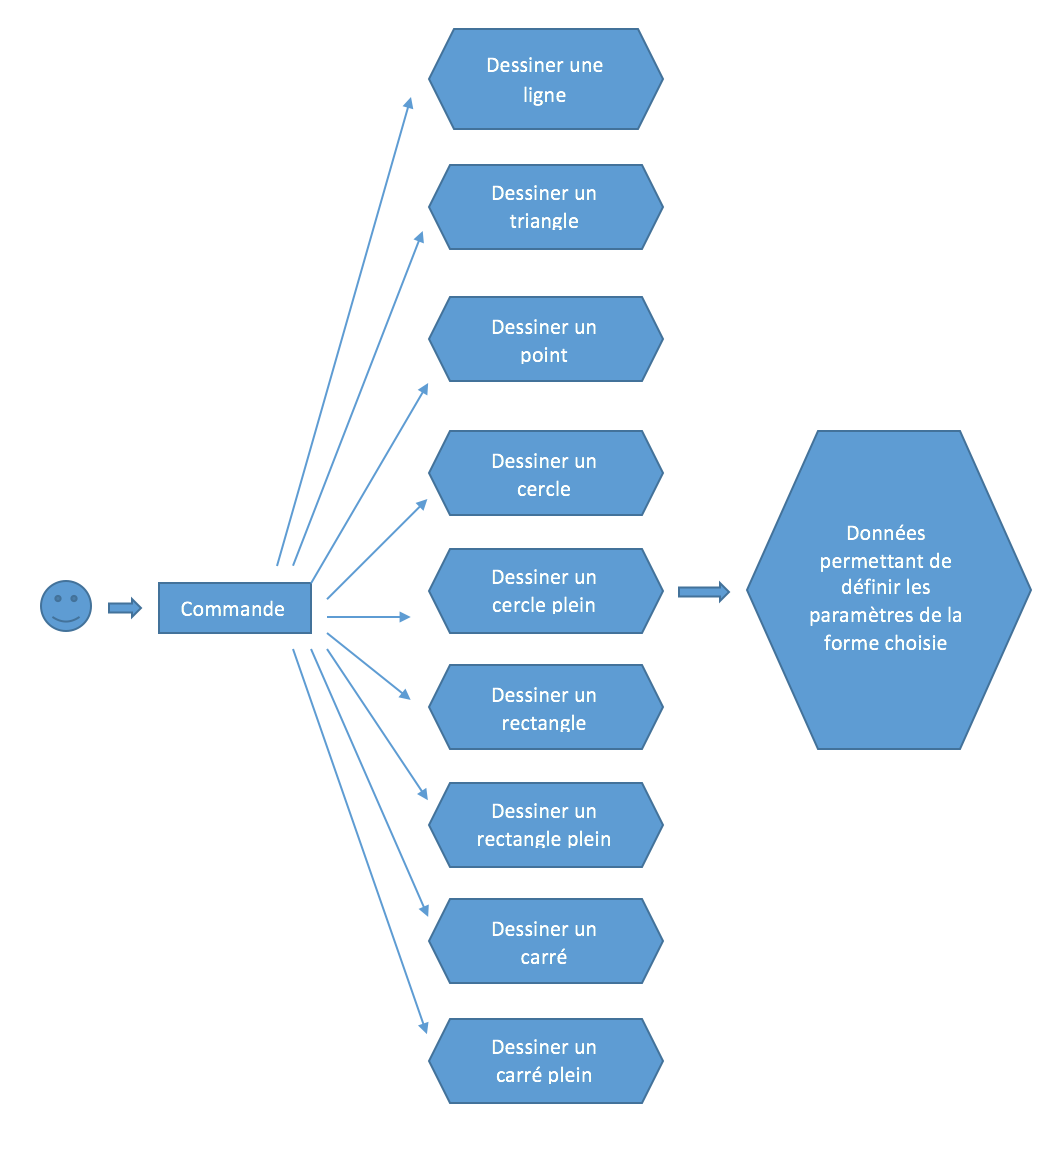
\includegraphics[width=16cm]{Photo1.png}
        \caption[Diagramme des cas d'utilisation]{Diagramme de cas d'utilisation de notre programme \texttt{dessin\_vect}}
    \centering
    \end{center}
\end{figure}

\clearpage

\subsection{Diagramme UML}

Le langage UML est un langage de modélisation graphique à base de pictogrammes conçu pour fournir une méthode simple pour visualiser la conception d'un système. Nous avons donc utilisé ce langage afin de nous permettre de suivre un cheminement clair et détaillé de notre projet. Ce diagramme permet aussi de comprendre comment les différentes classes ont été construites les unes par rapport aux autres, comme les rapports d'héritage. \\

\begin{figure}[!htbp]
    \begin{center}
        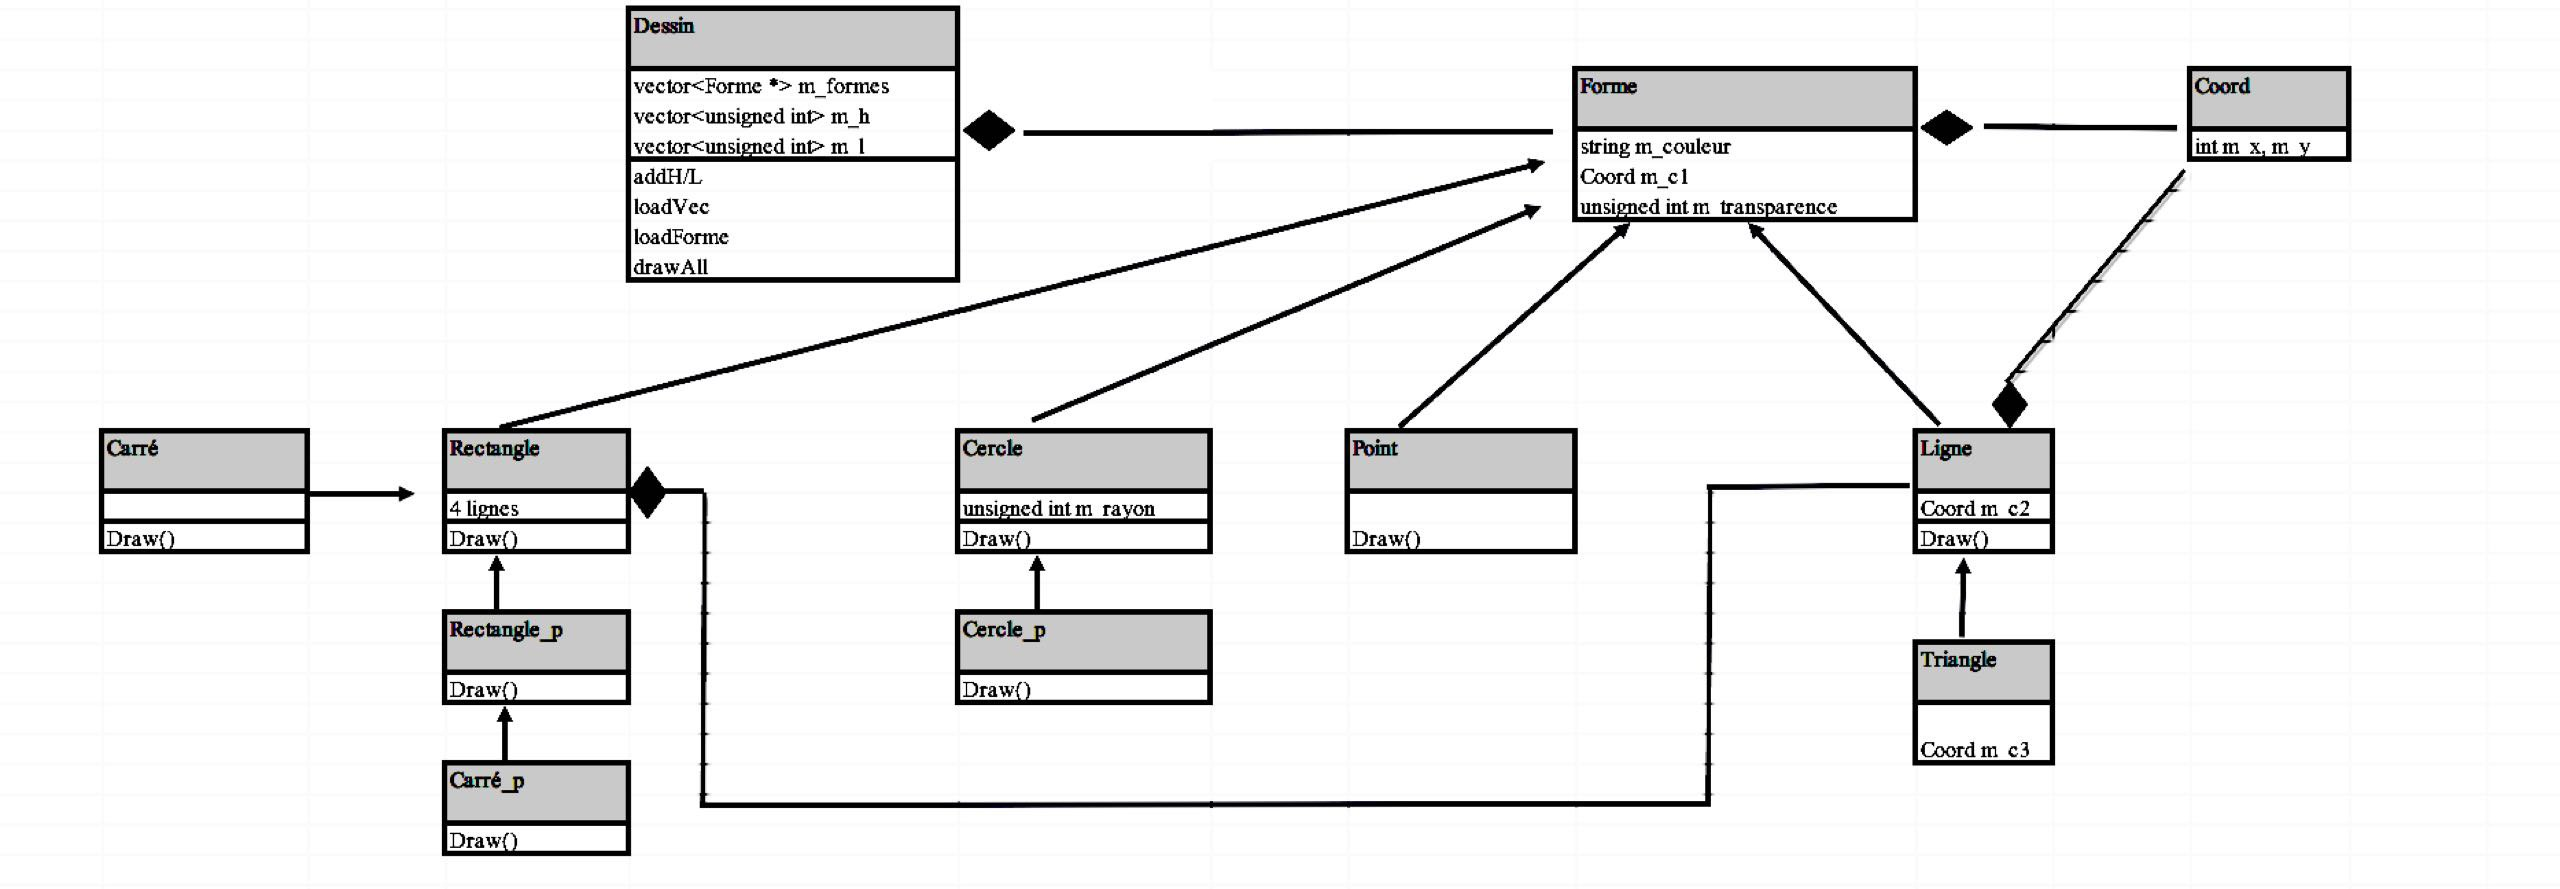
\includegraphics[width=20cm]{UML1.jpg}
        \caption{diagramme UML}
    \centering
    \end{center}
\end{figure}

Le diagramme UML fonctionne comme suit : 
\begin{itemize}
    \item Chaque classe utilisée est explicitée. Les attributs et les méthodes principales y figurent et leurs rapports d'héritage y sont expliqués. 
    \item Quand une classe en utilise une autre comme type d'attribut, un losange et une ligne font le lien entre les deux (le losange est placé sur la classe qui utilise l'autre comme type d'attribut).
    \item quand une classe hérite d'une autre, une flèche indique la classe mère et part de la classe fille. \\
\end{itemize}

D'autres classes - fournies par l'encadrant du projet - sont utilisées dans le projet : CBitmap gère la création d'un fichier bitmap (\texttt{.bmp}) à partie d'un objet CImage. CImage créé l'image dans laquelle on va dessiner avec la classe Dessin. On écrit dans CImage soit pixel par pixel (ce que l'on a choisi de faire). Un méthode publique à d’ailleurs été rajoutée dans CImage pour dessiner sur un pixel d'un simple appel de fonction. Les classes en question sont explicitées dans la figure suivante : 

\begin{figure}[!htbp]
    \begin{center}
        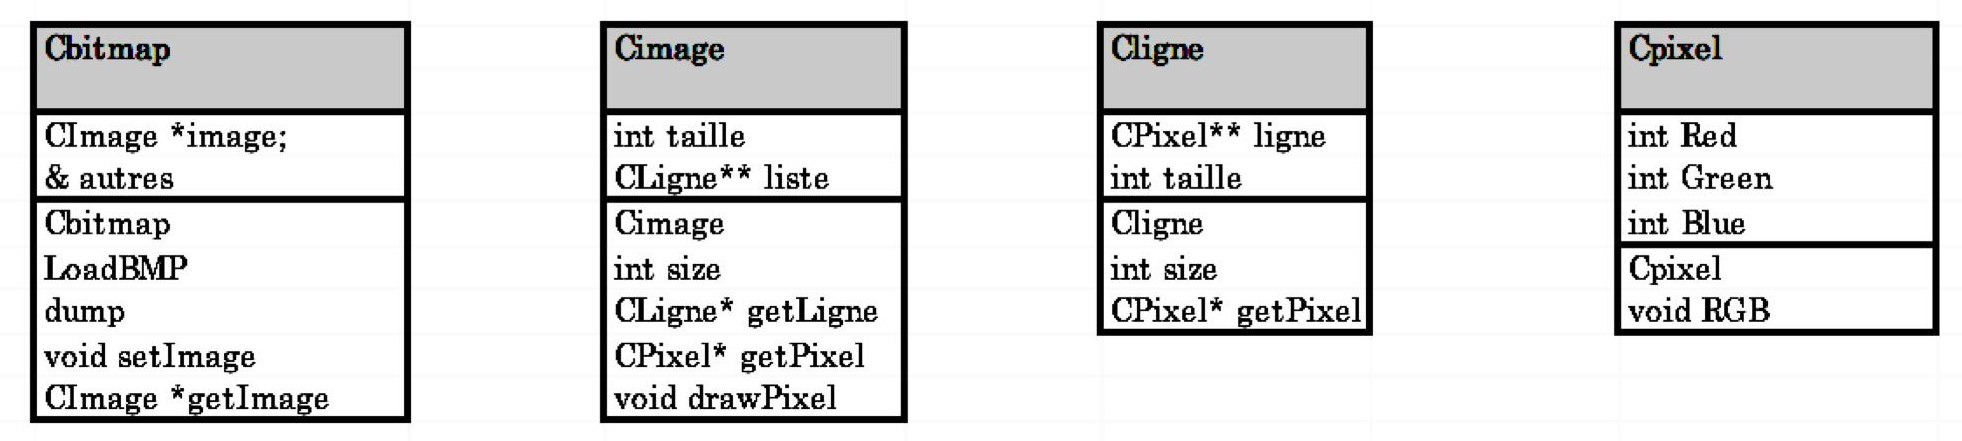
\includegraphics[width = 12cm]{UML2.jpg}
        \caption{Classes fournies par l'encadrant : CBitmap, CImage, CLigne, CPixel}
    \end{center}
\end{figure}


\section{Les classes principales}

Grâce au diagramme UML vu précédemment, nous avons pu commencer à écrire le code de notre projet par les classes principales. En effet certaines des classes à programmer sont plus importantes que d'autres. Nous avons fait le choix de créer une classe de coordonnées Coord (non indispensable mais qui nous a permis de nous approprier la notion de position d'un objet dans l'image dès le début) qui rassemble les coordonnées x et y de chaque forme. \\

Nous avons commencé par concevoir la classe forme contient tous les attributs communs aux futures classes des différentes formes. 

Ensuite, nous avons écrit le reste des classes de formes, en commençant par la classe Ligne. Celle-ci est à la base de beaucoup de formes. Par exemple, la méthode \texttt{drawLigne()} est utilisée dans toutes les formes (mis à part la classe Cercle et la classe Cercle\_p).

Enfin une classe Dessin permet de réunir toutes les formes en un seul objet, de définir les bornes de l'image, et de fournir les informations au dessin de l'image. 

\subsection{Classe de coordonnées Coord}

La classe \texttt{Coord} est une classe pratique. Celle-ci ne génère pas une forme, mais permet simplement de généraliser les 2 coordonnées d'un point en un seul objet. Cet objet servira d'attribut pour la classe Forme, ainsi que pour d'autres formes. 

\subsection{Classe forme Forme}

La classe mère Forme regroupe l'ensemble des attributs communs à toutes les classes de formes :

\begin{itemize}
    \item Coord m\_c1 : Cette coordonnée définit la position dans l'image de l'objet. Ce point sert de base pour construire le reste de la forme. 
    \item string m\_couleur : La couleur de l'objet. Tous les objets à dessiner doivent avoir une couleur définie, de manière à écrire cette couleur sur un pixel de l'image. Pour ce faire un format RGB est utilisé (0 à 255 pour chacune des trois couleur primordiales). 
    \item unsigned int m\_transparence : Ce facteur permet de définir le niveau de transparence de la forme sur le dessin.\\ 
\end{itemize}

Elle regroupe également les méthodes utilisées dans les différentes formes, c'est à dire la méthode générant la couleur des pixels en fonction des valeurs de R, G et B. De cette façon il nous est possible de récupérer la valeur de R, G et B indépendamment afin de déterminer la couleur de notre pixel. 

\begin{rmq}
    Nous avons rajouté une fonction \texttt{drawPixel} dans la classe CImage qui nous permet de dessiner chaque pixel grâce à un simple appel à cette fonction. 
\end{rmq}

Une des méthodes de la classe Forme nous permet de déterminer le réglage de la couleur du pixel en fonction du niveau de transparence retenu grâce à la formule suivante qui prends en arguments la position du pixel, la couleur à affecter, le niveau de transparence et la couleur du pixel avant application de la nouvelle couleur.  

$$Pixel'(x, y) = \frac{(100 - transparence).Pixel(x, y) + transparence.CouleurForme}{100}$$

\subsection{Classe Dessin}

La classe Dessin est la classe qui englobe toutes les formes dans le but de les dessiner. En revanche, elle à également d'autres fonctions. 

Elle est d'abord composée d'un vecteur de pointeur vers des objets de type Forme. Grâce à ce vecteur, on peut rassembler toutes les formes à dessiner dans un seul objet en vue de les traiter. En effet, toutes les formes héritent justement de la classe Forme, et donc un pointeur vers un objet de type Forme peut pointer vers un objet de type Cercle par exemple. Une fois que toutes les formes sont pointées par des éléments du vecteur \texttt{m\_formes}, un simple appel à la méthode \texttt{drawAll()} de la classe Dessin permet de dessiner l'ensemble de l'image dans l'objet de type CImage (classe fournie par le professeur encadrant). \\

La classe Dessin permet également de capitaliser les informations relatives aux positions extremum des différentes formes dans des attributs réservés pour cela. \texttt{m\_l} et \texttt{m\_h} sont des vecteurs d'entiers positifs recensant ces extremums. Après avoir trié ces vecteurs avec un tri à bulles, on peux en extraire le maximum et ainsi obtenir la hauteur et la largeur de l'image de destination. \\

Enfin, deux méthodes permettent de charger les informations vectorielles des formes depuis un fichier \texttt{.vec}. D'abord, \texttt{loadVec} est une méthode publique de Dessin qui prends en argument le nom du fichier \texttt{.vec}, en extrait une à une les lignes puis les passe en argument à la méthode privée \texttt{loadForme}. Cette dernière extrait toutes les informations d'une ligne et ajoute la forme correspondante au vecteur de pointeurs de type Forme de la classe Dessin. 

\clearpage

\begin{rmq}
    Les fichiers \texttt{.vec} peuvent contenir des commentaires. Les commentaires doivent avoir en premier caractère le "\#". En revanche, la gestion des lignes vides dans un fichier \texttt{.vec} n'est pas assuré dans cette version de \texttt{dessin\_vect}. 
\end{rmq}

\section{Classes filles de Forme}

\subsection{Classe Ligne}

La classe Ligne hérite de la classe Forme. En plus des attributs provenant de Forme, un autre objet de type Coord permet de définir la deuxième extrémité de la ligne. 

Quant à la ligne dans l'image, nous avons décidé de tracer nos lignes à l'aide de l’algorithme généralisé optimisé de Bresenham. Cette méthode permet d’identifier le sens du tracé de la ligne et de déterminer les pixels que l'on doit dessiner afin de s'approcher le plus près possible d'une ligne droite (avec un taux d'erreurs le plus faible possible). Pour cela, nous séparons l'écran en octants. Nous partons d'un point central, puis nous prenons le deuxième point de la ligne et nous calculons les deltas de la droite reliant ces deux points. Grâce à ceux-ci nous déterminons dans quel octant nous nous trouvons et appliquons ainsi l'algorithme de Bresenham dans cet octant. \\

\begin{figure}[!htbp]
    \begin{center}
        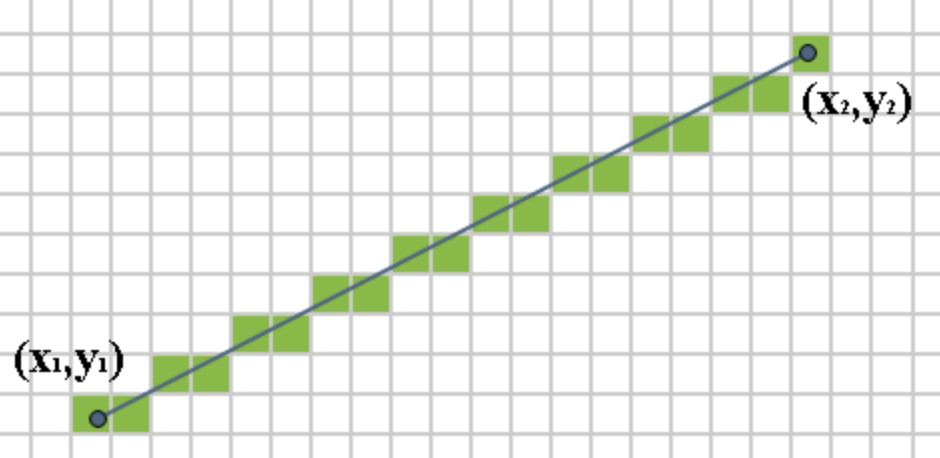
\includegraphics[width=8cm]{Photo3.png}
        \caption{Schéma explicatif de la méthode de Bresenham}
    \centering
    \end{center}
\end{figure}

\subsection{Le Point}

Le point hérite de la classe Forme. La seule chose qui diffère de Forme est la fonction \texttt{draw} qui permet de dessiner le point. Dans ce projet, le choix qui à été fait quand au dessin du point est de colorier un simple pixel à la coordonnée \texttt{m\_c1}. 

\begin{rmq}
    De part notre choix de la méthode de dessin du point, quand un facteur d'échelle est défini la position du point sera impacté mais pas sa taille. 
\end{rmq}

\subsection{Le cercle}

\subsubsection{Le cercle vide : Cercle}

Le cercle hérite de la classe Forme. Un attribut supplémentaire est défini dans Cercle : le rayon \texttt{m\_rayon}. Nous utilisons ensuite une condition de longueur, telle que si l'on se trouve à une distance r du centre, alors le pixel est dessiné. Afin d'avoir un tracé suffisamment large à l’œil humain, nous avons ajouté un "epsilon" de sorte que le pixel soit dessiné si il se trouve dans l’intervalle défini : $r \pm \varepsilon$

\subsubsection{Le cercle plein : Cercle\_p}

Le cercle plein Cercle\_p hérite de Cercle. Pour le dessiner, on dessine des cercles concentriques de rayon se décrémentant de \texttt{m\_rayon} jusqu'à 1. Ensuite on colorie un simple pixel au centre du cercle. 

\subsection{Le rectangle}

\subsubsection{Le rectangle vide : Rectangle}

Le rectangle vide hérite de Forme et est tout simplement créé à partir de 4 lignes. Ces lignes trouvent leurs coordonnées en fonction du point de départ (coin en bas à gauche du rectangle) et des longueurs et hauteurs. Pour le dessiner, il suffit de dessiner les 4 lignes qui sont en attribut. 

\subsubsection{Rectangle plein : Rectangle\_p}

Le rectangle plein hérite du rectangle simple et fonctionne à partir de lignes également. En effet, le remplissage se fait en balayant le rectangle dans la hauteur et en dessinant une ligne à chaque incrémentation. En revanche, on ne déclare pas d'objet Ligne à chaque incrémentation. 

\subsection{Le carré}

\subsubsection{Le carré vide : Carre}

La classe Carre hérite de la classe Rectangle. Pour le construire, on appelle le constructeur de Rectangle avec une hauteur égale à sa longueur. Pour le dessiner, la méthode est la même que pour la classe Rectangle. 

\subsubsection{Le carré plein : Carre\_p}

La classe Carre\_p hérite de la classe Rectangle\_p. Pour le construire, on appelle le constructeur de Rectangle\_p avec une hauteur égale à sa longueur. Pour le dessiner, la méthode est la même que pour la classe Rectangle\_p. 


\subsection{Le Triangle \texttt{Triangle}}

La classe Triangle hérite de la classe Ligne. Le seul attribut supplémentaire est un troisième objet Coord. Pour le dessiner, on créer les lignes manquantes et on dessine toutes les lignes. 

\section{Dimensions graphiques et facteur d'échelle}

Pour régler les dimensions de l'image de destinations, nous prenons les vecteurs d'extremums de Dessin (attributs \texttt(m\_l) et \texttt{m\_h}) et nous en extrayons le maximum. Ensuite, on adapte les bornes de notre objet CImage à partir de ces maximums est les passant en argument du constructeur de CImage. Ces extremums sont obtenus lors du chargement des objets dans la méthode \texttt{Dessin::loadForme}. \\

D'ailleurs, avant de récupérer les extremums, on les multiplie par le facteur d'échelle. De cette façon il est appliqué avant la définition des bornes de l'image et le dessin des formes. Le facteur d'échelle est un des arguments de l’exécutable. 

\section{Utilisation de notre programme \texttt{dessin\_vect}}

\subsection{Écriture du fichier .vec}

Pour utiliser notre programme, il faut d'abord écrire un fichier de description des formes. Chaque forme à un format particulier. Pour chaque forme, le format est le suivant : 

\begin{itemize}
    \item Le point : \texttt{PIXEL:600,600,BLANC,100}. Le mot clé POINT peut également être utilisé. Les arguments sont : x, y, couleur, transparence. 
    \item La ligne : \texttt{LIGNE:300,300,500,400,BLANC,100}. Le mot clé LINE peut également utilisé. Les arguments sont : x0, y0, x1, y1, couleur, transparence. 
    \item Le rectangle : \texttt{RECTANGLE:300,300,100,200,ROSE,100}. Les arguments sont : x, y, hauteur, largeur, couleur, transparence. 
    \item Le rectangle plein : \texttt{RECTANGLEP:300,300,30,50,MARRON,100}. Le mot clé RECTANGLES peut également être utilisé. Les arguments sont : x, y, hauteur, largeur, couleur, transparence. 
    \item Le carré : \texttt{CARRE:900,10,75,PINK,70}. Les arguments sont : x, y, hauteur, cote, transparence. 
    \item Le carré plein : \texttt{CARRES:900,10,75,PINK,70}. Le mot clé CARREP peut également être utilisé. Les arguments sont : x, y, hauteur, cote, transparence. 
    \item Le cercle : \texttt{CERCLE:500,500,75,ROSE,30}. Les arguments sont les suivants : x, y, rayon, couleur, transparence
    \item Le cercle plein : \texttt{CERCLEP:500,500,75,ROSE,30}. Les mots clé CERCLES et DISQUES peut également être utilisé. Les arguments sont : x, y, rayon, couleur, transparence
    \item Le triangle : \texttt{TRIANGLE:100,100,200,200,100,300,BLUE,100}. Les arguments sont : x1, y1, x2, y2, x3, y3, couleur, transparence. 
\end{itemize}

\subsection{Exécution du programme}

Une fois le programme compilé, on l’exécute avec la commande et les arguments suivants : 

\begin{center}
\texttt{\$ <chemin\_vers\_executable>/dessin\_vect <chemin\_vers\_.vec/nom.vec> <facteur d'échelle>}
\end{center}

\clearpage

\subsection{Résultats obtenus lors d'essais}

Voici deux images que nous avons obtenus lors des essais de notre programme final. 

\begin{figure}[!htbp]
    \begin{center}
        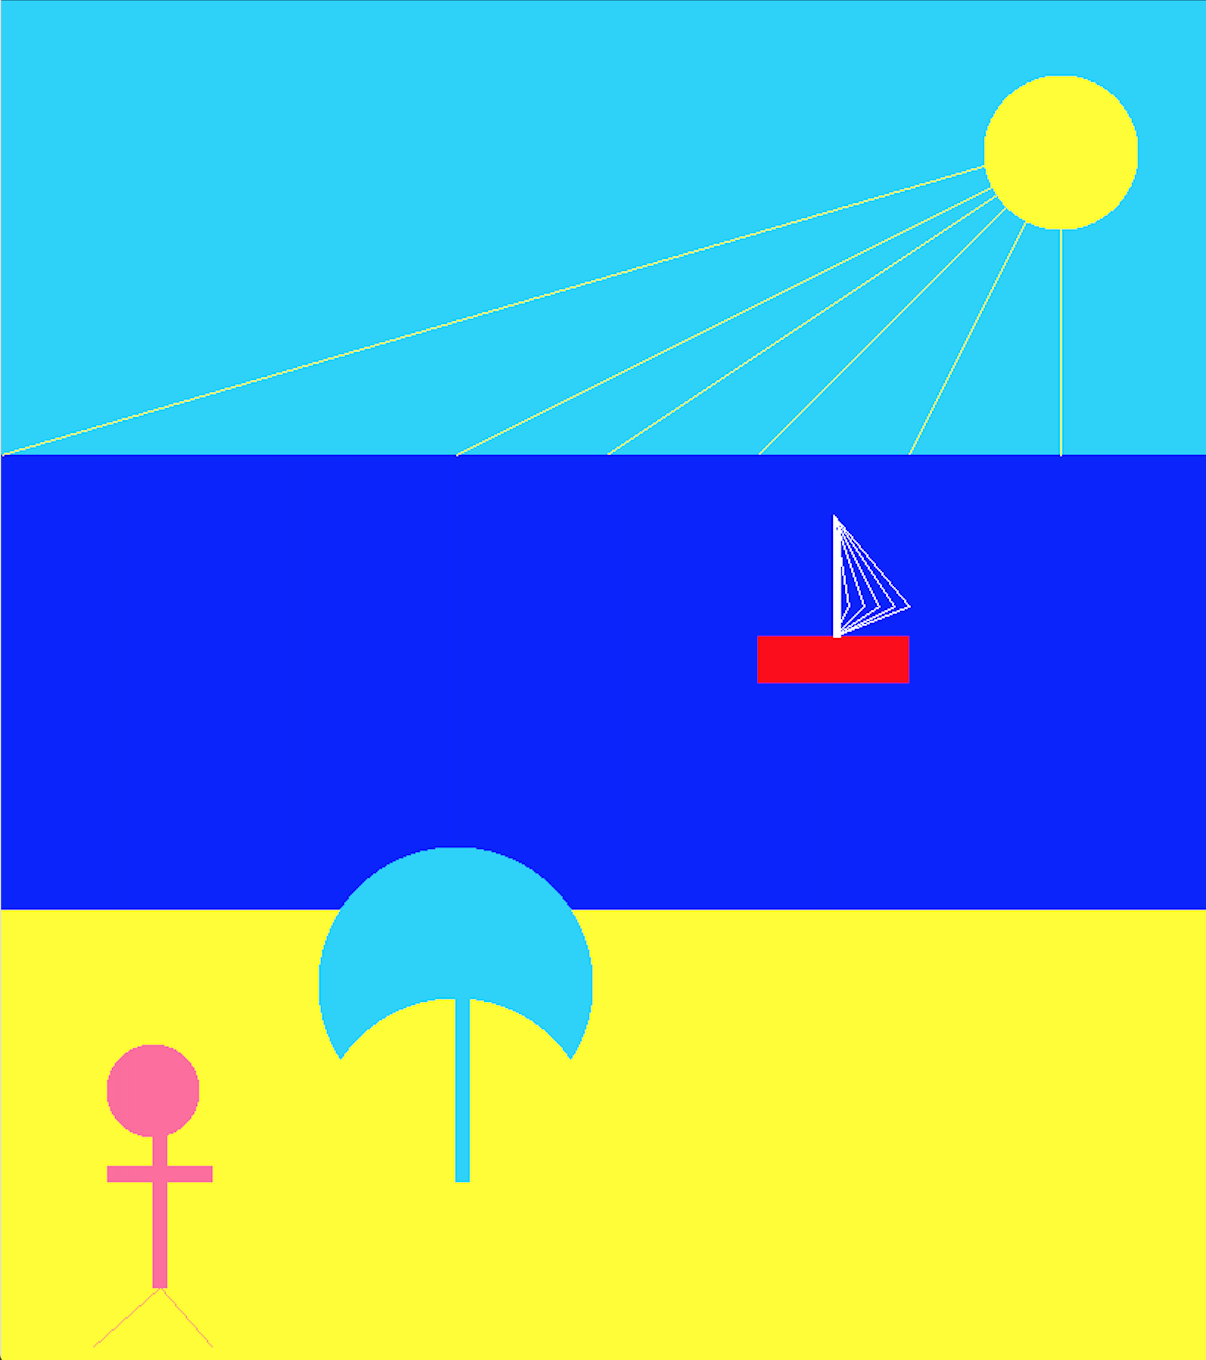
\includegraphics[width = 8cm]{plage.jpg}
        \caption{\texttt{plage.jpg}}
    \end{center}
\end{figure}

\begin{figure}[!htbp]
    \begin{center}
        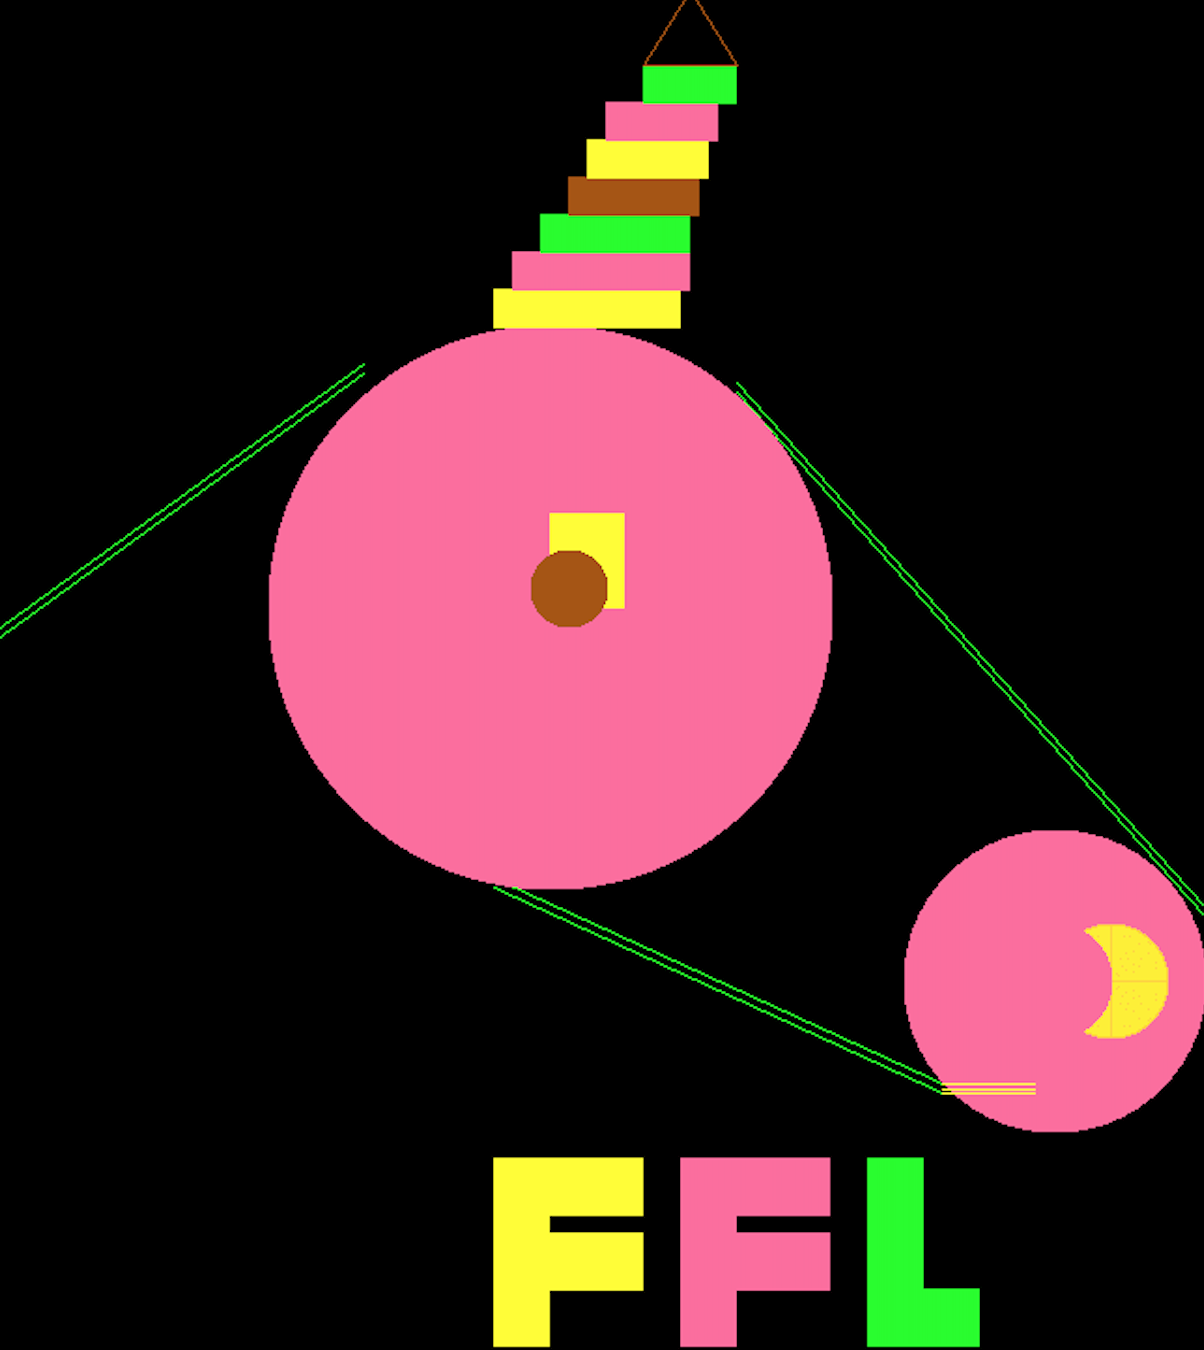
\includegraphics[width = 8cm]{licorne.jpg}
        \caption{licorne.jpg}
    \end{center}
\end{figure}

\clearpage

\section{Conclusion}

Ce projet nous a permis d'avoir un aperçu sur les possibilités que nous offre le langage C++. En effet celui celui-ci est un réel avantage quant à la programmation objet. Nous parvenons ainsi à dessiner dans un fichier bitmap des images à partir d'une description vectorielle des formes qui la compose. Néanmoins il est possible d'approfondir ce projet tant dans les formes disponibles (nous nous sommes intéressés au rectangle de travers par exemple) que dans une interface plus ergonomique, comme une interface graphique par exemple.

\end{document}